En el Aprendizaje Automático (Machine Learning), es vital distinguir entre las variables que el modelo aprende por sí solo y las configuraciones que el científico de datos debe establecer manualmente.

\subsubsection{1. Parámetros (Lo que la máquina aprende)}
Son las variables internas del modelo cuyos valores se ajustan automáticamente a partir de los datos durante el proceso de entrenamiento. El programador no los define directamente.
\begin{itemize}
    \item \textbf{Origen:} Se estiman y optimizan mediante el algoritmo (ej. Descenso del Gradiente).
    \item \textbf{Ejemplos:} Los coeficientes ($\beta$) en una regresión lineal, los vectores de soporte en SVM, o los pesos ($w$) y sesgos ($b$) en una red neuronal.
\end{itemize}

\subsection{2. Hiperparámetros (Lo que el humano configura)}
Son las variables de configuración externas que definen la ``arquitectura'' del modelo o cómo se comportará el algoritmo de aprendizaje. Deben fijarse \textbf{antes} de que comience el entrenamiento.
\begin{itemize}
    \item \textbf{Origen:} Los define empíricamente el científico de datos o mediante técnicas de búsqueda (Grid Search, Random Search).
    \item \textbf{Ejemplos:} La tasa de aprendizaje (\textit{learning rate}), el número de capas ocultas en una red neuronal, el valor de $K$ en K-Medias, o la profundidad máxima de un árbol de decisión.
\end{itemize}

\vspace{0.5cm}
\subsection{Ejemplo Gráfico: Red Neuronal}

En el siguiente gráfico se ilustra una red neuronal sencilla para visualizar visualmente dónde reside un hiperparámetro y dónde reside un parámetro.

\begin{figure}[H]
    \centering
    \shorthandoff{>} % Previene conflictos con babel español
    \resizebox{0.85\textwidth}{!}{%
    \begin{tikzpicture}[
        neuron/.style = {circle, draw, thick, minimum size=1.1cm, font=\large},
        input/.style = {neuron, fill=blue!15, draw=blue!80!black},
        hidden/.style = {neuron, fill=orange!15, draw=orange!80!black},
        output/.style = {neuron, fill=green!15, draw=green!80!black},
        connect/.style = {->, >=stealth, thick, draw=gray!60},
        highlight/.style = {->, >=stealth, very thick, draw=red}
    ]
    % ================= Capas de la Red =================
    % Capa de Entrada
    \node[input] (I1) at (0, 2.2) {$x_1$};
    \node[input] (I2) at (0, -2.2) {$x_2$};
    % Capa Oculta (Espaciada verticalmente)
    \node[hidden] (H1) at (3, 2.5) {$h_1$};
    \node[hidden] (H2) at (3, 0) {$h_2$};
    \node[hidden] (H3) at (3, -2.5) {$h_3$};
    % Capa de Salida
    \node[output] (O) at (6, 0) {$\hat{y}$};
    % ================= Títulos de las Capas =================
    \node[above=0.4cm of I1, font=\bfseries\small, text=blue!80!black] {Entrada};
    \node[above=0.4cm of H1, font=\bfseries\small, text=orange!80!black] {Capa Oculta};
    \node[above=0.4cm of O, font=\bfseries\small, text=green!80!black] {Salida};
    % ================= Conexiones =================
    \foreach \i in {1,2}
        \foreach \h in {1,2,3}
            \draw[connect] (I\i) -- (H\h);
    \draw[connect] (H1) -- (O);
    \draw[highlight] (H2) -- (O); % Conexión del parámetro
    \draw[connect] (H3) -- (O);
    % ================= Etiquetas de Conceptos =================
    % PARÁMETRO: Flotando limpiamente arriba de la línea roja
    % LÍNEA CORREGIDA:
    \node[text=red, font=\bfseries\small, align=center] at (4.5, 0.4) {Parámetro:\\Peso $w$};    % HIPERPARÁMETROS: Caja elegante posicionada abajo, sin tocar la red
    \node[draw=orange!60, fill=orange!5, rounded corners, thick, inner sep=0.3cm, font=\small, align=left] 
        at (3, -4.8) (hyperbox) {
        \textbf{\color{orange!80!black} Hiperparámetros (Configuración estructural definida previamente):} \\
        $\bullet$ Número de capas ocultas = 1 \quad $\bullet$ Neuronas por capa = 3 \quad $\bullet$ Tasa de aprendizaje ($\alpha$) = 0.01
    };
    \end{tikzpicture}%
    }
    \caption{Diseño limpio del modelo: Los hiperparámetros dictan la estructura global que se muestra abajo, mientras que el parámetro (peso $w$) es un valor interno que el algoritmo calcula de forma precisa para la conexión.}
    \label{fig:params_vs_hyper_clean}
\end{figure}

\subsection{Árboles de Decisión (Decision Trees)}
Este modelo segmenta el espacio de características mediante reglas de decisión condicionales, estructuradas de forma jerárquica.

\begin{itemize}
    \item \textbf{El Algoritmo:} Evalúa de forma iterativa todas las variables para encontrar el punto de corte óptimo que maximice la homogeneidad de los subgrupos resultantes, utilizando métricas como la Ganancia de Información o el Índice Gini.
    \item \textbf{El Modelo:} Es una estructura en árbol donde los nodos internos representan preguntas lógicas y las hojas contienen las predicciones finales.
\end{itemize}

\begin{figure}[htbp]
    \centering
    \shorthandoff{>}
    \resizebox{0.7\textwidth}{!}{%
    \begin{tikzpicture}[
        node distance = 1.2cm and 1.5cm,
        root/.style = {rectangle, draw=purple!80!black, fill=purple!10, thick, rounded corners, minimum width=2.5cm, minimum height=1cm, font=\small\sffamily, align=center},
        decision/.style = {rectangle, draw=blue!80!black, fill=blue!10, thick, rounded corners, minimum width=2.5cm, minimum height=1cm, font=\small\sffamily, align=center},
        leaf/.style = {ellipse, draw=green!80!black, fill=green!10, thick, minimum width=2cm, font=\small\sffamily, align=center}
    ]
        % Nodos del árbol
        \node[root] (root) {¿Ingresos $>$ \$3000?};
        \node[decision, below left=1cm and 1.5cm of root] (d1) {¿Es menor de 30 años?};
        \node[leaf, below right=1cm and 1.5cm of root] (l1) {\textbf{Aprobar Crédito}};
        \node[leaf, below left=1.2cm and 0.5cm of d1] (l2) {\textbf{Rechazar Crédito}};
        \node[leaf, below right=1.2cm and 0.5cm of d1] (l3) {\textbf{Aprobar Crédito}};

        % Conexiones
        \draw[->, >=stealth, thick] (root) -- node[above left, font=\footnotesize] {No} (d1);
        \draw[->, >=stealth, thick] (root) -- node[above right, font=\footnotesize] {Sí} (l1);
        \draw[->, >=stealth, thick] (d1) -- node[above left, font=\footnotesize] {Sí} (l2);
        \draw[->, >=stealth, thick] (d1) -- node[above right, font=\footnotesize] {No} (l3);
    \end{tikzpicture}%
    }
    \caption{Estructura matemática de un Árbol de Decisión: Un flujo jerárquico de particiones lógicas.}
    \label{fig:decision_tree}
\end{figure}

\subsection{Modelos de Mezcla Gaussiana (GMM)}
Es un modelo de agrupamiento probabilístico que asume que los datos provienen de una combinación lineal de múltiples distribuciones normales independientes.

\begin{itemize}
    \item \textbf{El Algoritmo:} Utiliza el método iterativo de \textbf{Expectación-Maximización (EM)} para aproximar de forma óptima la ubicación y dispersión de las densidades probabilísticas.
    \item \textbf{El Modelo:} Matemáticamente se expresa como una densidad de probabilidad conjunta:
\end{itemize}
\begin{equation}
    p(x) = \sum_{k=1}^{K} \pi_k \mathcal{N}(x \mid \mu_k, \Sigma_k)
\end{equation}
\textit{(Donde $\pi_k$ representa el peso o importancia de la mezcla, $\mu_k$ el centro o media, y $\Sigma_k$ la matriz de covarianza que define la forma geométrica del grupo $k$).}

\begin{figure}[htbp]
    \centering
    \shorthandoff{>}
    \resizebox{0.55\textwidth}{!}{%
    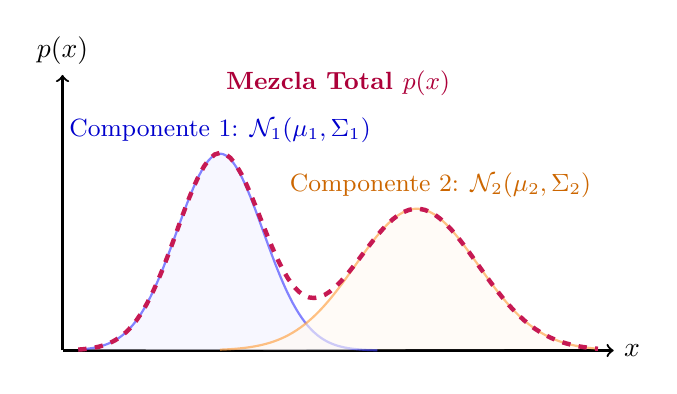
\begin{tikzpicture}
        % Dibujo de curvas gaussianas solapadas
        \draw[->, thick] (-3,0) -- (4,0) node[right] {$x$};
        \draw[->, thick] (-3,0) -- (-3,3.5) node[above] {$p(x)$};
        
        % Gaussiana 1 (Izquierda)
        \draw[thick, blue!80, fill=blue!5, opacity=0.6, domain=-2.8:1, samples=100] 
            plot (\x, {2.5*exp(-(\x+1)*(\x+1)/0.6)});
        \node[blue!80!black, font=\small] at (-1, 2.8) {Componente 1: $\mathcal{N}_1(\mu_1, \Sigma_1)$};
        
        % Gaussiana 2 (Derecha)
        \draw[thick, orange!80, fill=orange!5, opacity=0.6, domain=-1:3.8, samples=100] 
            plot (\x, {1.8*exp(-(\x-1.5)*(\x-1.5)/1.2)});
        \node[orange!80!black, font=\small] at (1.8, 2.1) {Componente 2: $\mathcal{N}_2(\mu_2, \Sigma_2)$};
        
        % Línea de densidad combinada (Suma)
        \draw[ultra thick, purple!90, dashed, domain=-2.8:3.8, samples=100] 
            plot (\x, {2.5*exp(-(\x+1)*(\x+1)/0.6) + 1.8*exp(-(\x-1.5)*(\x-1.5)/1.2)});
        \node[purple!90!black, font=\bfseries\small] at (0.5, 3.4) {Mezcla Total $p(x)$};
    \end{tikzpicture}%
    }
    \caption{Representación de un GMM: Distribuciones probabilísticas continuas que se superponen para modelar densidades complejas.}
    \label{fig:gmm_plot}
\end{figure}

\begin{table}[htbp]
\centering
\caption{Identificación de Parámetros e Hiperparámetros por Modelo}
\vspace{0.2cm}
\begin{tabular}{|l|p{5cm}|p{5cm}|}
\hline
\textbf{Modelo} & \textbf{Hiperparámetros} \newline (Tus decisiones previas) & \textbf{Parámetros} \newline (Lo que el modelo aprendió) \\ \hline
\textbf{Red Neuronal} & Número de capas, neuronas por capa, tasa de aprendizaje ($\alpha$). & Pesos ($w$) de las conexiones y sesgos ($b$). \\ \hline
\textbf{Árbol de Decisión} & Profundidad máxima del árbol, criterio de división (Gini/Entropía). & Variables seleccionadas para los nodos y umbrales de corte (ej: \$3000). \\ \hline
\textbf{GMM} & Número de componentes o grupos a buscar ($K$). & Medias ($\mu$), covarianzas ($\Sigma$) y pesos de cada campana ($\pi$). \\ \hline
\end{tabular}
\end{table}